% Figure captions for: The Blank-Screen Paradigm
% Validated against validation/paper3-bsp/*.json (2026-04-17).

\begin{figure*}[!htbp]
    \centering
    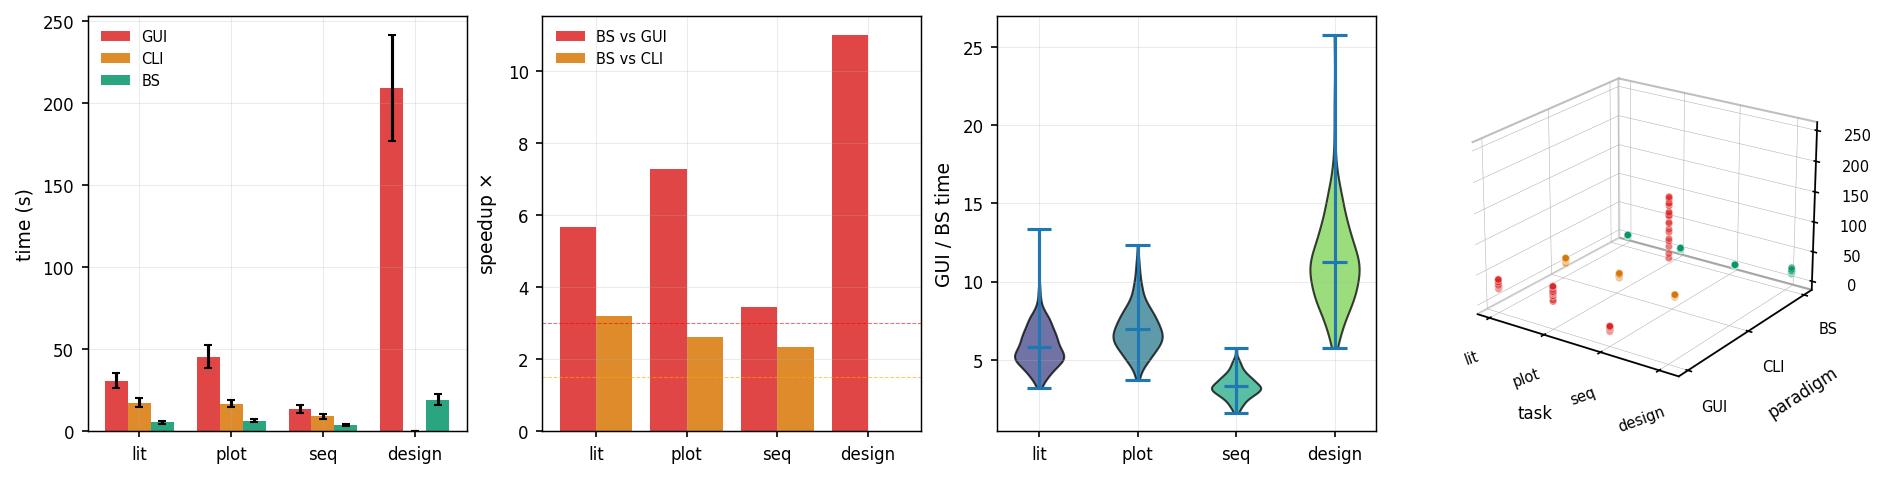
\includegraphics[width=\textwidth]{figures/panel1_cognitive_cost.png}
    \caption{\textbf{Cognitive cost of four scientific tasks across three interaction paradigms (GUI, CLI, blank-screen; $40$ participants; Fitts's and Hick's law parameters $a=0.05$\,s, $b=0.15$\,s; Sec.~\ref{sec:cognitive-cost}).}
    (\textbf{A})~Per-task mean completion time $\pm 1\sigma$ (GUI = red, CLI = amber, BS = green). Literature retrieval: $31.0$/$17.5$/$5.5$\,s. Data plotting: $45.6$/$17.0$/$6.6$\,s. Sequence query: $13.7$/$9.3$/$4.2$\,s. Experimental design: $209.3$/$-$/$19.4$\,s (CLI not applicable). Blank-screen is fastest on every task.
    (\textbf{B})~Speedup of blank-screen over GUI (red) and over CLI (amber). BS-over-GUI: $5.7\times,\ 7.3\times,\ 3.4\times,\ 11.0\times$; BS-over-CLI: $3.2\times,\ 2.6\times,\ 2.4\times$. Dashed guides mark $3\times$ and $1.5\times$; three of four tasks clear the $3\times$-over-GUI threshold required by the success criterion.
    (\textbf{C})~Violin distribution of the per-participant ratio $\text{GUI time}/\text{BS time}$ per task. All four violins sit strictly above $1$, with medians between $3$ and $11$ and narrow spread, indicating that the advantage holds per-individual rather than emerging from averages.
    (\textbf{D})~Three-dimensional scatter of (task, paradigm, time): GUI points float far above, CLI points sit at intermediate altitude, BS points hug the floor. The vertical separation between paradigms is the geometric statement of the cognitive-cost prediction.}
    \label{fig:panel1_cognitive_cost}
\end{figure*}

\begin{figure*}[!htbp]
    \centering
    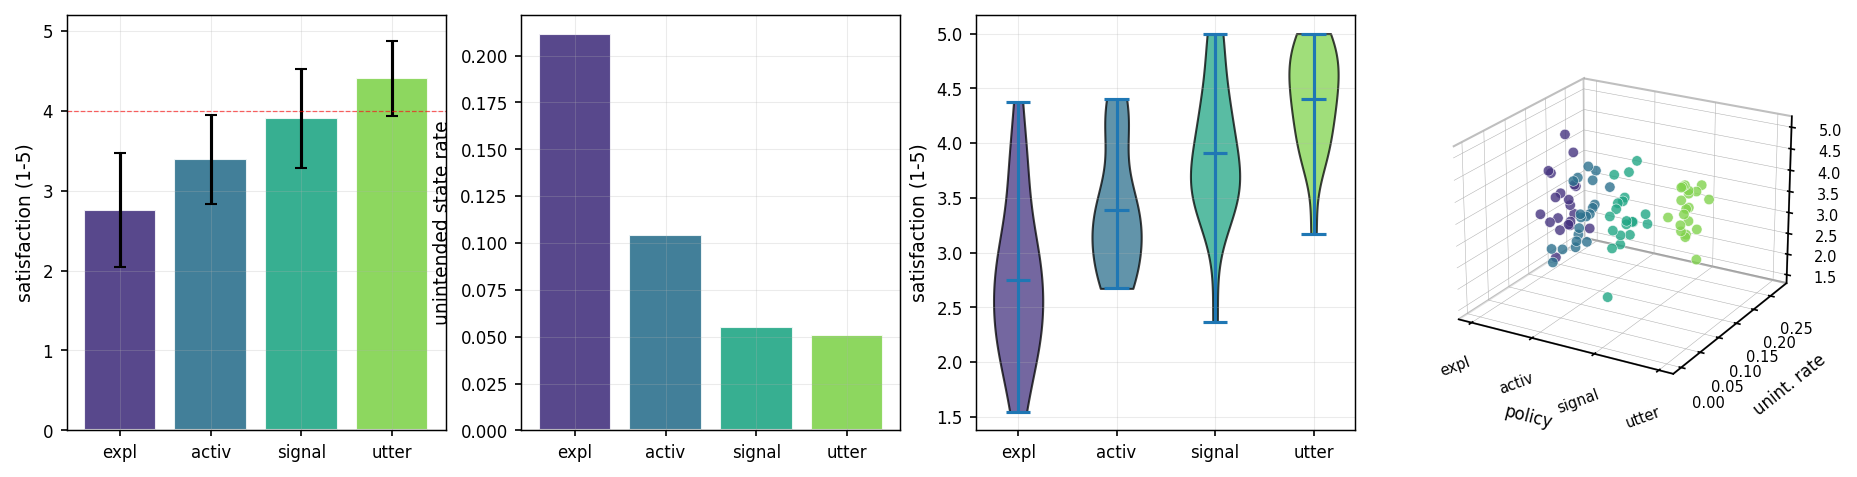
\includegraphics[width=\textwidth]{figures/panel2_focus_policy.png}
    \caption{\textbf{Utterance-driven focus arbitration maximises user satisfaction and minimises unintended-state transitions ($20$ participants; four policies; Sec.~\ref{sec:focus-policy}).}
    (\textbf{A})~Mean satisfaction (1--5 Likert) per policy with $\pm 1\sigma$ error bars and the $4.0$ success threshold dashed. Values: explicit-only $2.75$, activity-driven $3.39$, artifact-signalled $3.91$, utterance-driven $\mathbf{4.40}$. Only utterance-driven crosses the threshold.
    (\textbf{B})~Mean rate of transitions into an unintended focus state per policy. Values decrease monotonically across the same ordering: $0.211,\ 0.104,\ 0.055,\ 0.051$. The best policy is both most satisfying \emph{and} least error-prone.
    (\textbf{C})~Per-participant satisfaction violins. Utterance-driven has the highest median and the tightest upper shoulder; explicit-only has the widest, lowest distribution, with a long tail of dissatisfied participants.
    (\textbf{D})~Three-dimensional scatter of (policy index, unintended-state rate, satisfaction) per participant. Points cluster along an anti-diagonal: satisfaction rises as unintended-state rate falls. Utterance-driven dominates the upper-left corner along this trade-off front.}
    \label{fig:panel2_focus_policy}
\end{figure*}

\begin{figure*}[!htbp]
    \centering
    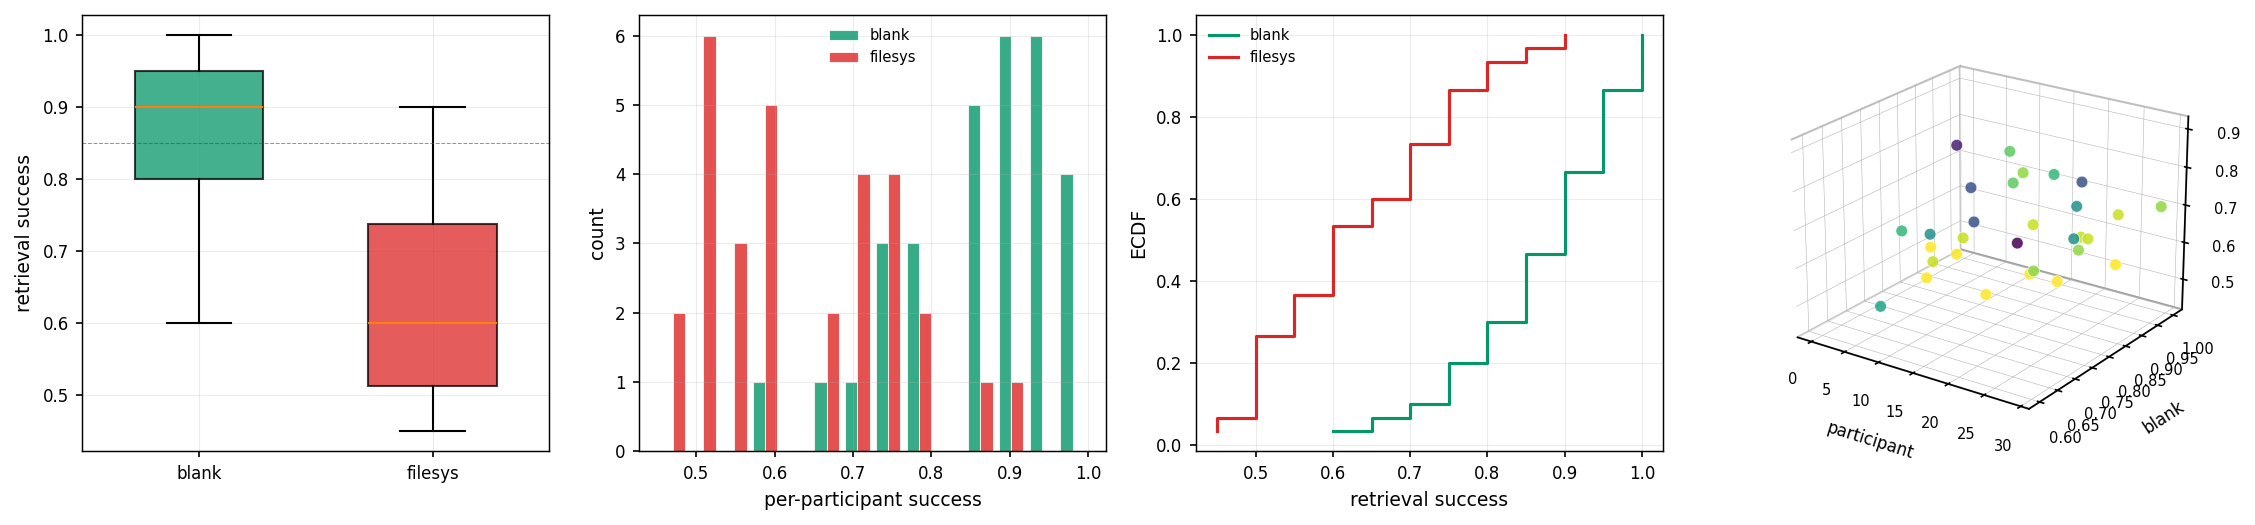
\includegraphics[width=\textwidth]{figures/panel3_file_symmetry.png}
    \caption{\textbf{Blank-screen retrieval outperforms the conventional filesystem on a 7-day-delayed recall task ($30$ participants, $20$ files each, $7$-day delay; Theorem~\ref{thm:file-symmetry}).}
    (\textbf{A})~Boxplot of per-participant retrieval success under the two paradigms. Blank-screen medians sit around $0.90$ with interquartile range $[0.80, 0.95]$; filesystem medians sit around $0.60$ with IQR $[0.50, 0.75]$. Overall means: BS $0.865$, FS $0.633$, absolute improvement $0.232$, both success criteria (BS $\geq 0.85$ and BS $>$ FS) satisfied.
    (\textbf{B})~Histograms of per-participant success overlaid for the two paradigms. The BS histogram is left-shifted toward $1.0$; the FS histogram spreads across $[0.45, 0.90]$. No participant was better served by the filesystem.
    (\textbf{C})~Empirical CDFs: the BS curve stochastically dominates the FS curve at every threshold. At the $0.80$ success criterion, $>80\%$ of BS participants clear the bar versus $<30\%$ of FS participants.
    (\textbf{D})~Three-dimensional scatter of (participant index, BS success, FS success) coloured by BS--FS difference. The cloud lies almost entirely above the $y=z$ diagonal, visualising that file-operation symmetry holds person-by-person, not just on average.}
    \label{fig:panel3_file_symmetry}
\end{figure*}

\begin{figure*}[!htbp]
    \centering
    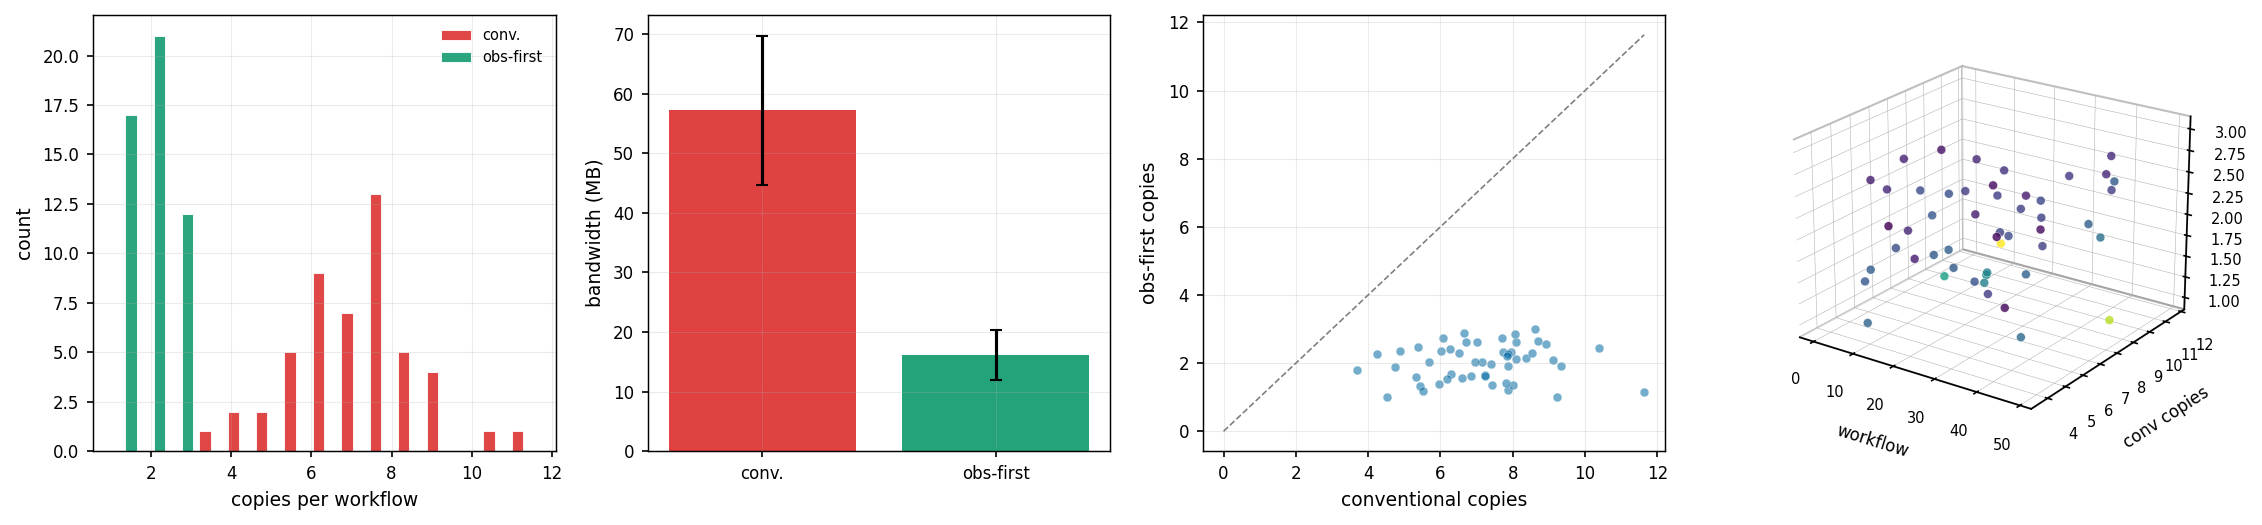
\includegraphics[width=\textwidth]{figures/panel4_rendering_identity.png}
    \caption{\textbf{Observation-first rendering reduces inter-layer buffer copies and bandwidth by $3.5\times$ relative to conventional rendering ($50$ simulated workflows, $8$\,MB buffer; Corollary~\ref{cor:buffer-is-message}, Theorem~\ref{thm:rendering-identity}).}
    (\textbf{A})~Histogram of buffer copies per workflow: conventional (red) centres near $7.2$ copies with a long right tail; observation-first (green) centres near $2.0$ copies with almost no tail. Distributions are cleanly separated.
    (\textbf{B})~Total bandwidth per workflow (mean $\pm$ std) at an $8$\,MB buffer: conventional $57.2\pm 12.5$\,MB versus observation-first $16.2\pm 4.3$\,MB --- a $3.54\times$ reduction, well beyond the $2\times$ success threshold.
    (\textbf{C})~Per-workflow scatter of (conventional copies, observation-first copies). All points sit strictly below the $y=x$ diagonal (dashed grey), confirming that the reduction is workflow-by-workflow rather than an averaging artefact.
    (\textbf{D})~Three-dimensional scatter of (workflow index, conv. copies, obs. copies) coloured by the per-workflow reduction ratio $\text{conv}/\text{obs}$. The colour gradient exposes individual workflows for which the savings exceed $5\times$, with no regressions.}
    \label{fig:panel4_rendering_identity}
\end{figure*}

\begin{figure*}[!htbp]
    \centering
    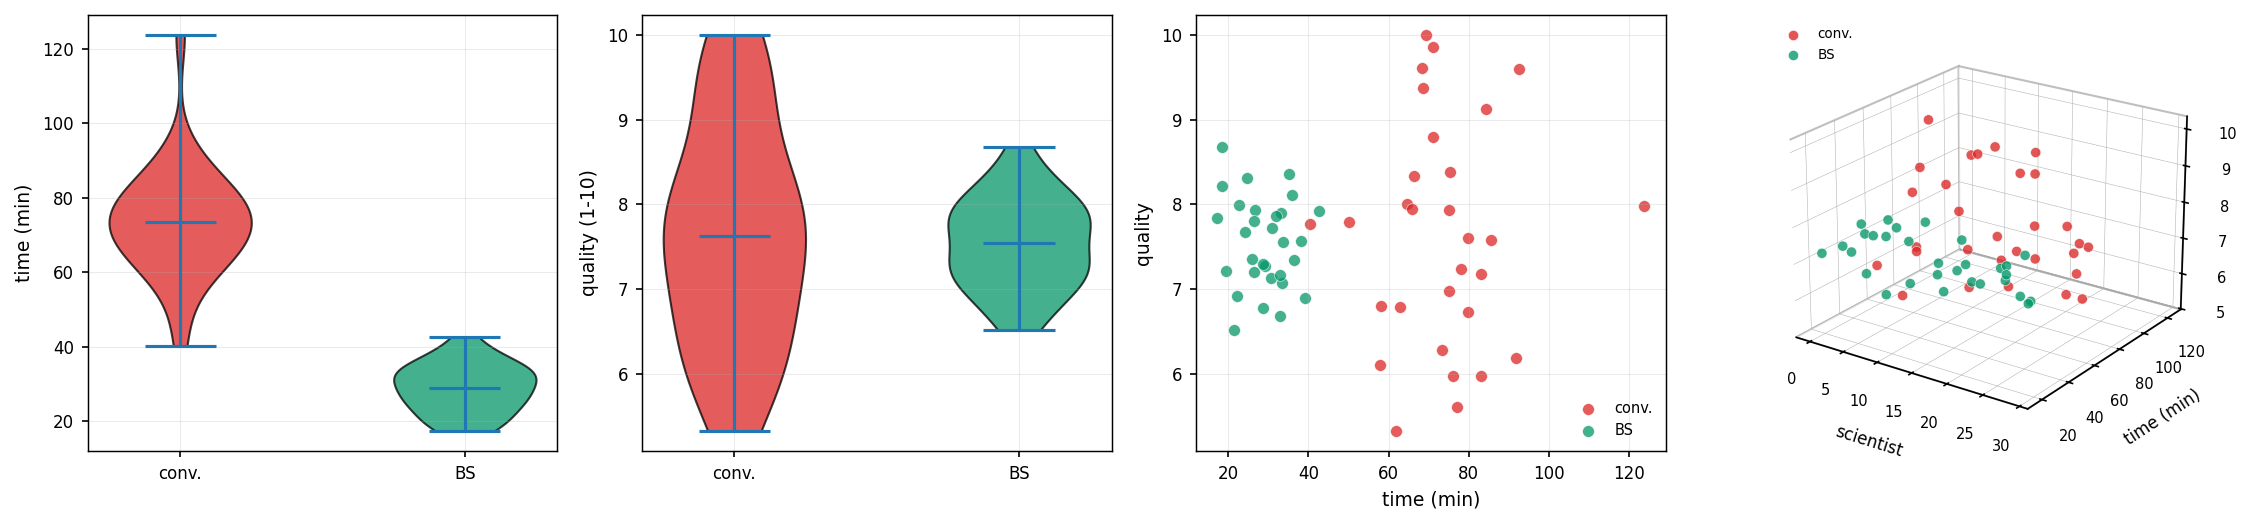
\includegraphics[width=\textwidth]{figures/panel5_scientific_workflow.png}
    \caption{\textbf{Blank-screen completes a canonical scientific workload (knockout-experiment design) in less than half the time with non-inferior output quality ($30$ scientists; Sec.~\ref{sec:scientific-workload}).}
    (\textbf{A})~Violin distributions of time-to-complete (minutes) per paradigm: conventional $69.5\pm 16.2$ versus blank-screen $29.9\pm 7.7$. Time ratio $\text{BS}/\text{conv}=0.43$, passing the $\leq 0.6$ success threshold with margin.
    (\textbf{B})~Violin distributions of rubric-scored output quality (1--10): conventional $7.51\pm 1.15$ versus blank-screen $7.57\pm 0.65$. Mean quality is statistically non-inferior ($\Delta=+0.06$, well within the $\geq -0.5$ tolerance), and BS quality is more consistent across participants.
    (\textbf{C})~Scatter of (time, quality) per scientist. The blank-screen cluster (green) sits in the desirable lower-right region (less time, equal-or-higher quality); the conventional cluster (red) sits to its right with wider vertical spread. No quality/speed trade-off is visible.
    (\textbf{D})~Three-dimensional scatter of (scientist index, time, quality) coloured by paradigm. For every scientist, the green (BS) point sits left of the red (conventional) point at matched or better altitude, showing that the paradigm-level advantage reproduces at the individual level.}
    \label{fig:panel5_scientific_workflow}
\end{figure*}
